\section{Diseño de la Solución}

\subsection{Arquitectura del Sistema}
La solución se compone de tres capas arquitectónicas:
\begin{enumerate}
    \item \textbf{Capa Primaria (Controladores y Presentación):} Servidor HTTP en Go que expone una interfaz gráfica HTML/CSS/JS y una API REST compatible con OpenAPI 3.0.
    \item \textbf{Capa de Aplicación y Dominio:} Servicios orquestadores transaccionales que coordinan la creación de recursos y gestionan fallos mediante rutinas de compensación (\textit{rollback}).
    \item \textbf{Capa Secundaria (Adaptadores de Infraestructura):} Implementaciones concretas de los puertos que invocan la interfaz de línea de comandos de VirtualBox (\texttt{VBoxManage}), utilitarios DNS (\texttt{nsupdate} o SSH sobre Bind9) y utilidades de transferencia de archivos.
\end{enumerate}

\subsection{Topología de Red}
Se define una red interna virtual (\texttt{cloudnet}) bajo el segmento IPv4 \texttt{192.168.10.0/24}:
\begin{itemize}
    \item \textbf{Host anfitrión:} \texttt{192.168.10.1} (interfaz Host-Only).
    \item \textbf{Servidor DNS (\texttt{ns}):} \texttt{192.168.10.10/24}, administrando la zona \texttt{cloud.local.}.
    \item \textbf{Instancias dinámicas:} Direcciones en el rango \texttt{192.168.10.30} a \texttt{192.168.10.254}.
\end{itemize}

\begin{figure}[htbp]
\centering
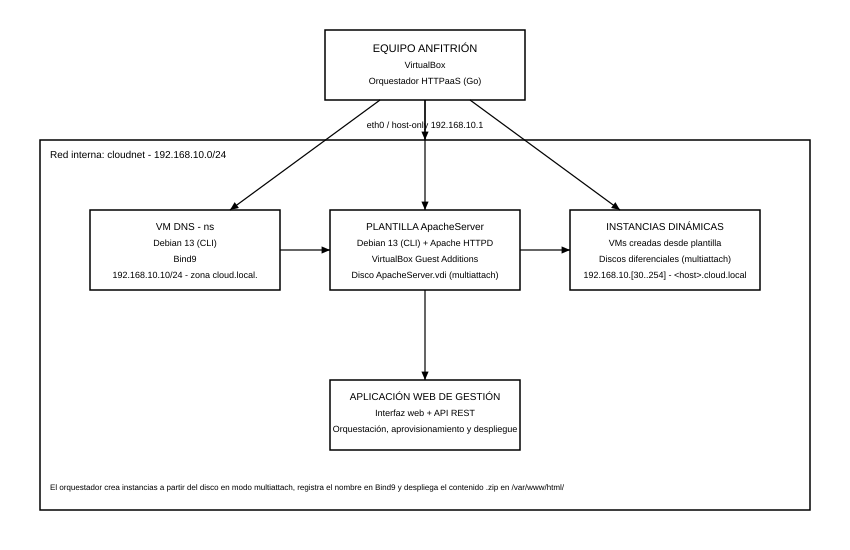
\includegraphics[width=\linewidth]{escenario.svg}
\caption{Diagrama de escenario: topología de red y componentes del entorno HTTPaaS.}
\label{fig:escenario}
\end{figure}



\subsection{Vista de Procesos: Flujo de Aprovisionamiento}
El aprovisionamiento se realiza de forma automatizada y transaccional, garantizando la coherencia entre los componentes de virtualización, DNS y despliegue web.

\begin{figure}[htbp]
\centering
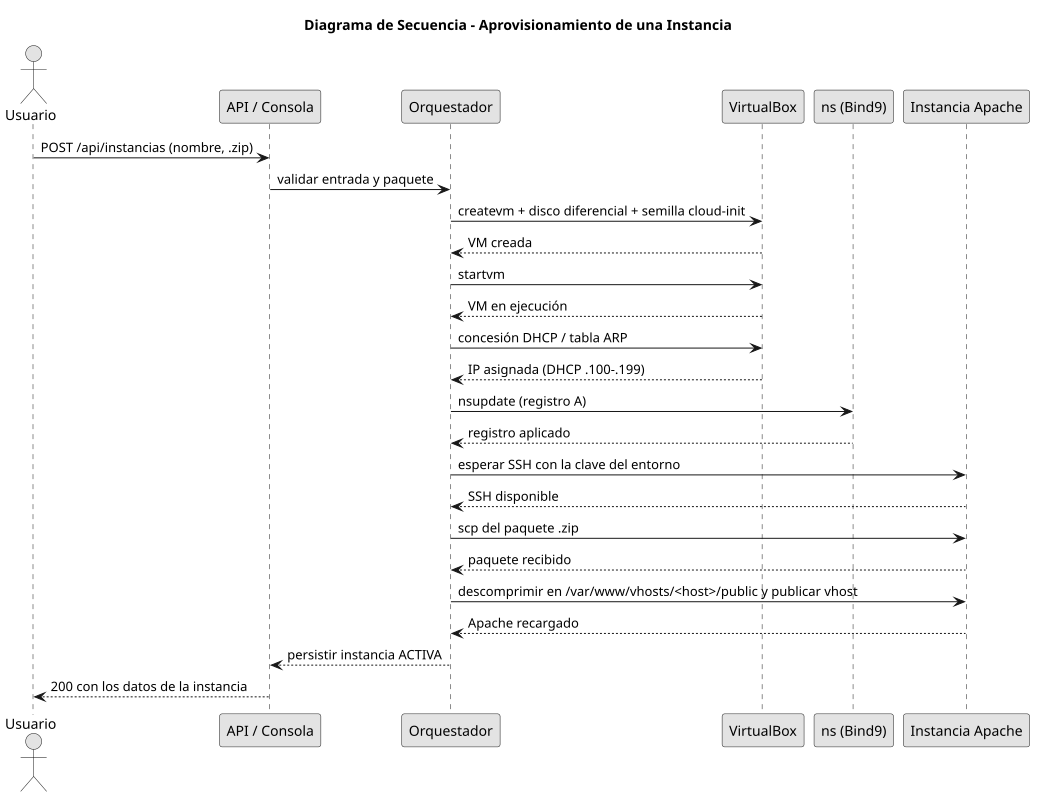
\includegraphics[width=\linewidth]{secuencia.svg}
\caption{Diagrama de secuencia del flujo de aprovisionamiento de instancias HTTPaaS.}
\label{fig:secuencia}
\end{figure}

\subsection{Manejo de Compensaciones (Rollback)}
Si alguna etapa del aprovisionamiento falla, el orquestador ejecuta rutinas de compensación inversa para mantener la infraestructura en un estado consistente:
\begin{itemize}
    \item Si falla el registro DNS: se destruye la máquina virtual creada en VirtualBox.
    \item Si falla el despliegue del archivo \texttt{.zip}: se elimina el registro DNS correspondiente y se destruye la máquina virtual creada en VirtualBox.
\end{itemize}
